\documentclass[]{article}
\usepackage{lmodern}
\usepackage{amssymb,amsmath}
\usepackage{ifxetex,ifluatex}
\usepackage{fixltx2e} % provides \textsubscript
\ifnum 0\ifxetex 1\fi\ifluatex 1\fi=0 % if pdftex
  \usepackage[T1]{fontenc}
  \usepackage[utf8]{inputenc}
\else % if luatex or xelatex
  \ifxetex
    \usepackage{mathspec}
  \else
    \usepackage{fontspec}
  \fi
  \defaultfontfeatures{Ligatures=TeX,Scale=MatchLowercase}
\fi
% use upquote if available, for straight quotes in verbatim environments
\IfFileExists{upquote.sty}{\usepackage{upquote}}{}
% use microtype if available
\IfFileExists{microtype.sty}{%
\usepackage{microtype}
\UseMicrotypeSet[protrusion]{basicmath} % disable protrusion for tt fonts
}{}
\usepackage[margin=1in]{geometry}
\usepackage{hyperref}
\hypersetup{unicode=true,
            pdftitle={Homework 01},
            pdfauthor={Marco Zullich},
            pdfborder={0 0 0},
            breaklinks=true}
\urlstyle{same}  % don't use monospace font for urls
\usepackage{color}
\usepackage{fancyvrb}
\newcommand{\VerbBar}{|}
\newcommand{\VERB}{\Verb[commandchars=\\\{\}]}
\DefineVerbatimEnvironment{Highlighting}{Verbatim}{commandchars=\\\{\}}
% Add ',fontsize=\small' for more characters per line
\usepackage{framed}
\definecolor{shadecolor}{RGB}{248,248,248}
\newenvironment{Shaded}{\begin{snugshade}}{\end{snugshade}}
\newcommand{\KeywordTok}[1]{\textcolor[rgb]{0.13,0.29,0.53}{\textbf{#1}}}
\newcommand{\DataTypeTok}[1]{\textcolor[rgb]{0.13,0.29,0.53}{#1}}
\newcommand{\DecValTok}[1]{\textcolor[rgb]{0.00,0.00,0.81}{#1}}
\newcommand{\BaseNTok}[1]{\textcolor[rgb]{0.00,0.00,0.81}{#1}}
\newcommand{\FloatTok}[1]{\textcolor[rgb]{0.00,0.00,0.81}{#1}}
\newcommand{\ConstantTok}[1]{\textcolor[rgb]{0.00,0.00,0.00}{#1}}
\newcommand{\CharTok}[1]{\textcolor[rgb]{0.31,0.60,0.02}{#1}}
\newcommand{\SpecialCharTok}[1]{\textcolor[rgb]{0.00,0.00,0.00}{#1}}
\newcommand{\StringTok}[1]{\textcolor[rgb]{0.31,0.60,0.02}{#1}}
\newcommand{\VerbatimStringTok}[1]{\textcolor[rgb]{0.31,0.60,0.02}{#1}}
\newcommand{\SpecialStringTok}[1]{\textcolor[rgb]{0.31,0.60,0.02}{#1}}
\newcommand{\ImportTok}[1]{#1}
\newcommand{\CommentTok}[1]{\textcolor[rgb]{0.56,0.35,0.01}{\textit{#1}}}
\newcommand{\DocumentationTok}[1]{\textcolor[rgb]{0.56,0.35,0.01}{\textbf{\textit{#1}}}}
\newcommand{\AnnotationTok}[1]{\textcolor[rgb]{0.56,0.35,0.01}{\textbf{\textit{#1}}}}
\newcommand{\CommentVarTok}[1]{\textcolor[rgb]{0.56,0.35,0.01}{\textbf{\textit{#1}}}}
\newcommand{\OtherTok}[1]{\textcolor[rgb]{0.56,0.35,0.01}{#1}}
\newcommand{\FunctionTok}[1]{\textcolor[rgb]{0.00,0.00,0.00}{#1}}
\newcommand{\VariableTok}[1]{\textcolor[rgb]{0.00,0.00,0.00}{#1}}
\newcommand{\ControlFlowTok}[1]{\textcolor[rgb]{0.13,0.29,0.53}{\textbf{#1}}}
\newcommand{\OperatorTok}[1]{\textcolor[rgb]{0.81,0.36,0.00}{\textbf{#1}}}
\newcommand{\BuiltInTok}[1]{#1}
\newcommand{\ExtensionTok}[1]{#1}
\newcommand{\PreprocessorTok}[1]{\textcolor[rgb]{0.56,0.35,0.01}{\textit{#1}}}
\newcommand{\AttributeTok}[1]{\textcolor[rgb]{0.77,0.63,0.00}{#1}}
\newcommand{\RegionMarkerTok}[1]{#1}
\newcommand{\InformationTok}[1]{\textcolor[rgb]{0.56,0.35,0.01}{\textbf{\textit{#1}}}}
\newcommand{\WarningTok}[1]{\textcolor[rgb]{0.56,0.35,0.01}{\textbf{\textit{#1}}}}
\newcommand{\AlertTok}[1]{\textcolor[rgb]{0.94,0.16,0.16}{#1}}
\newcommand{\ErrorTok}[1]{\textcolor[rgb]{0.64,0.00,0.00}{\textbf{#1}}}
\newcommand{\NormalTok}[1]{#1}
\usepackage{graphicx,grffile}
\makeatletter
\def\maxwidth{\ifdim\Gin@nat@width>\linewidth\linewidth\else\Gin@nat@width\fi}
\def\maxheight{\ifdim\Gin@nat@height>\textheight\textheight\else\Gin@nat@height\fi}
\makeatother
% Scale images if necessary, so that they will not overflow the page
% margins by default, and it is still possible to overwrite the defaults
% using explicit options in \includegraphics[width, height, ...]{}
\setkeys{Gin}{width=\maxwidth,height=\maxheight,keepaspectratio}
\IfFileExists{parskip.sty}{%
\usepackage{parskip}
}{% else
\setlength{\parindent}{0pt}
\setlength{\parskip}{6pt plus 2pt minus 1pt}
}
\setlength{\emergencystretch}{3em}  % prevent overfull lines
\providecommand{\tightlist}{%
  \setlength{\itemsep}{0pt}\setlength{\parskip}{0pt}}
\setcounter{secnumdepth}{0}
% Redefines (sub)paragraphs to behave more like sections
\ifx\paragraph\undefined\else
\let\oldparagraph\paragraph
\renewcommand{\paragraph}[1]{\oldparagraph{#1}\mbox{}}
\fi
\ifx\subparagraph\undefined\else
\let\oldsubparagraph\subparagraph
\renewcommand{\subparagraph}[1]{\oldsubparagraph{#1}\mbox{}}
\fi

%%% Use protect on footnotes to avoid problems with footnotes in titles
\let\rmarkdownfootnote\footnote%
\def\footnote{\protect\rmarkdownfootnote}

%%% Change title format to be more compact
\usepackage{titling}

% Create subtitle command for use in maketitle
\providecommand{\subtitle}[1]{
  \posttitle{
    \begin{center}\large#1\end{center}
    }
}

\setlength{\droptitle}{-2em}

  \title{Homework 01}
    \pretitle{\vspace{\droptitle}\centering\huge}
  \posttitle{\par}
    \author{Marco Zullich}
    \preauthor{\centering\large\emph}
  \postauthor{\par}
      \predate{\centering\large\emph}
  \postdate{\par}
    \date{6 April 2019}


\begin{document}
\maketitle

\section{TH-1}\label{th-1}

To fit the model with uninformative prior using \texttt{bayesglm}. This
function assumes a Student-t prior distribution for the parameters,
hence, to reproduce a noninformative priors case, we need to set the
\texttt{prior.scale} parameter to infinite for both the slope and the
intercept, and \texttt{prior.df} to 1 (to produce a curve as flat as
possible). After fitting, we plot our dataset with the regression line
to visualize if it fits our data well.

\begin{Shaded}
\begin{Highlighting}[]
\NormalTok{(}\DataTypeTok{lm =}\NormalTok{ arm}\OperatorTok{::}\KeywordTok{bayesglm}\NormalTok{(}\StringTok{"dist~speed"}\NormalTok{, }\DataTypeTok{data=}\NormalTok{cars, }\DataTypeTok{prior.scale=}\OtherTok{Inf}\NormalTok{, }\DataTypeTok{prior.df =} \DecValTok{1}\NormalTok{, }\DataTypeTok{prior.scale.for.intercept =} \OtherTok{Inf}\NormalTok{, }\DataTypeTok{prior.df.for.intercept =} \DecValTok{1}\NormalTok{))}
\end{Highlighting}
\end{Shaded}

\begin{verbatim}
## 
## Call:  arm::bayesglm(formula = "dist~speed", data = cars, prior.scale = Inf, 
##     prior.df = 1, prior.scale.for.intercept = Inf, prior.df.for.intercept = 1)
## 
## Coefficients:
## (Intercept)        speed  
##     -17.579        3.932  
## 
## Degrees of Freedom: 49 Total (i.e. Null);  48 Residual
## Null Deviance:       32540 
## Residual Deviance: 11350     AIC: 419.2
\end{verbatim}

\begin{Shaded}
\begin{Highlighting}[]
\KeywordTok{plot}\NormalTok{(cars}\OperatorTok{$}\NormalTok{dist }\OperatorTok{~}\StringTok{ }\NormalTok{cars}\OperatorTok{$}\NormalTok{speed)}
\KeywordTok{abline}\NormalTok{(}\DataTypeTok{a=}\NormalTok{lm}\OperatorTok{$}\NormalTok{coefficients[}\DecValTok{1}\NormalTok{], }\DataTypeTok{b=}\NormalTok{lm}\OperatorTok{$}\NormalTok{coefficients[}\DecValTok{2}\NormalTok{], }\DataTypeTok{col=}\StringTok{"red"}\NormalTok{)}
\end{Highlighting}
\end{Shaded}

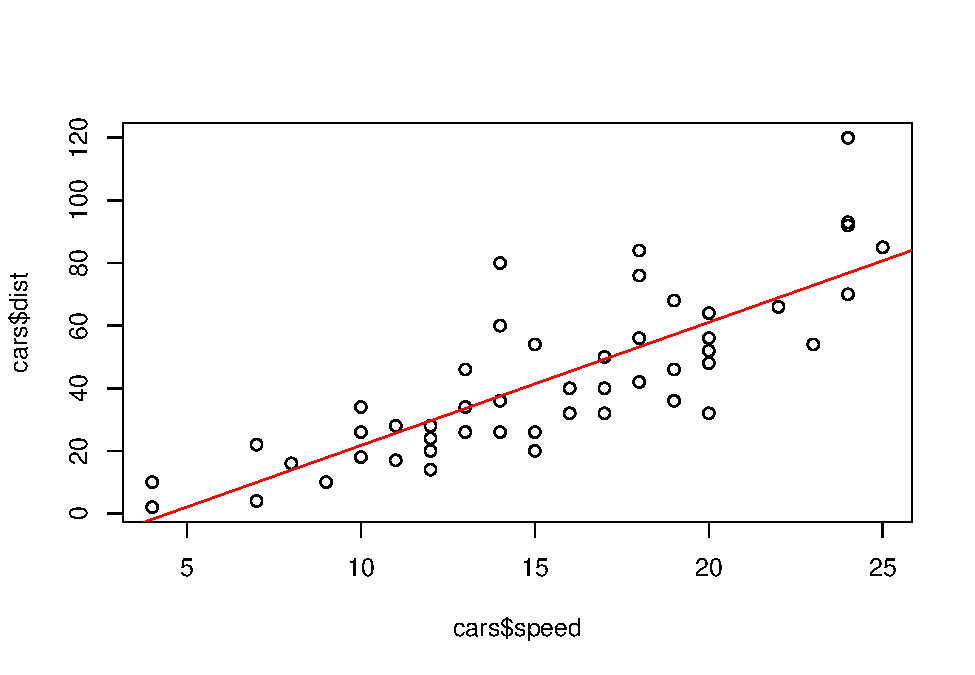
\includegraphics{ex01_files/figure-latex/unnamed-chunk-1-1.pdf}

To fit the informative model, instead, we just play with the parameters
of \texttt{bayesglm}

\begin{Shaded}
\begin{Highlighting}[]
\NormalTok{(}\DataTypeTok{lm_inf1 =}\NormalTok{ arm}\OperatorTok{::}\KeywordTok{bayesglm}\NormalTok{(}\StringTok{"dist~speed"}\NormalTok{, }\DataTypeTok{data=}\NormalTok{cars, }\DataTypeTok{prior.scale=}\DecValTok{1}\NormalTok{, }\DataTypeTok{prior.df =} \OtherTok{Inf}\NormalTok{, }\DataTypeTok{prior.scale.for.intercept =} \DecValTok{1}\NormalTok{, }\DataTypeTok{prior.df.for.intercept =} \OtherTok{Inf}\NormalTok{))}
\end{Highlighting}
\end{Shaded}

\begin{verbatim}
## 
## Call:  arm::bayesglm(formula = "dist~speed", data = cars, prior.scale = 1, 
##     prior.df = Inf, prior.scale.for.intercept = 1, prior.df.for.intercept = Inf)
## 
## Coefficients:
## (Intercept)        speed  
##     -17.652        3.932  
## 
## Degrees of Freedom: 49 Total (i.e. Null);  48 Residual
## Null Deviance:       32540 
## Residual Deviance: 11350     AIC: 419.2
\end{verbatim}

\begin{Shaded}
\begin{Highlighting}[]
\NormalTok{(}\DataTypeTok{lm_inf2 =}\NormalTok{ arm}\OperatorTok{::}\KeywordTok{bayesglm}\NormalTok{(}\StringTok{"dist~speed"}\NormalTok{, }\DataTypeTok{data=}\NormalTok{cars, }\DataTypeTok{prior.scale=}\NormalTok{.}\DecValTok{1}\NormalTok{, }\DataTypeTok{prior.df =} \OtherTok{Inf}\NormalTok{, }\DataTypeTok{prior.scale.for.intercept =}\NormalTok{ .}\DecValTok{1}\NormalTok{, }\DataTypeTok{prior.df.for.intercept =} \OtherTok{Inf}\NormalTok{))}
\end{Highlighting}
\end{Shaded}

\begin{verbatim}
## 
## Call:  arm::bayesglm(formula = "dist~speed", data = cars, prior.scale = 0.1, 
##     prior.df = Inf, prior.scale.for.intercept = 0.1, prior.df.for.intercept = Inf)
## 
## Coefficients:
## (Intercept)        speed  
##      -25.02         3.90  
## 
## Degrees of Freedom: 49 Total (i.e. Null);  48 Residual
## Null Deviance:       32540 
## Residual Deviance: 14510     AIC: 431.4
\end{verbatim}

\begin{Shaded}
\begin{Highlighting}[]
\NormalTok{(}\DataTypeTok{lm_inf3 =}\NormalTok{ arm}\OperatorTok{::}\KeywordTok{bayesglm}\NormalTok{(}\StringTok{"dist~speed"}\NormalTok{, }\DataTypeTok{data=}\NormalTok{cars, }\DataTypeTok{prior.mean =} \DecValTok{1}\NormalTok{, }\DataTypeTok{prior.scale=}\NormalTok{.}\DecValTok{2}\NormalTok{, }\DataTypeTok{prior.df =} \OtherTok{Inf}\NormalTok{, }\DataTypeTok{prior.mean.for.intercept =} \DecValTok{1}\NormalTok{, }\DataTypeTok{prior.scale.for.intercept =}\NormalTok{ .}\DecValTok{2}\NormalTok{, }\DataTypeTok{prior.df.for.intercept =} \OtherTok{Inf}\NormalTok{))}
\end{Highlighting}
\end{Shaded}

\begin{verbatim}
## 
## Call:  arm::bayesglm(formula = "dist~speed", data = cars, prior.mean = 1, 
##     prior.scale = 0.2, prior.df = Inf, prior.mean.for.intercept = 1, 
##     prior.scale.for.intercept = 0.2, prior.df.for.intercept = Inf)
## 
## Coefficients:
## (Intercept)        speed  
##     -19.317        3.928  
## 
## Degrees of Freedom: 49 Total (i.e. Null);  48 Residual
## Null Deviance:       32540 
## Residual Deviance: 11520     AIC: 419.9
\end{verbatim}

\begin{Shaded}
\begin{Highlighting}[]
\NormalTok{(}\DataTypeTok{lm_inf4 =}\NormalTok{ arm}\OperatorTok{::}\KeywordTok{bayesglm}\NormalTok{(}\StringTok{"dist~speed"}\NormalTok{, }\DataTypeTok{data=}\NormalTok{cars, }\DataTypeTok{prior.scale=}\NormalTok{.}\DecValTok{001}\NormalTok{, }\DataTypeTok{prior.df =} \OtherTok{Inf}\NormalTok{, }\DataTypeTok{prior.scale.for.intercept =}\NormalTok{ .}\DecValTok{001}\NormalTok{, }\DataTypeTok{prior.df.for.intercept =} \OtherTok{Inf}\NormalTok{))}
\end{Highlighting}
\end{Shaded}

\begin{verbatim}
## 
## Call:  arm::bayesglm(formula = "dist~speed", data = cars, prior.scale = 0.001, 
##     prior.df = Inf, prior.scale.for.intercept = 0.001, prior.df.for.intercept = Inf)
## 
## Coefficients:
## (Intercept)        speed  
##   -0.085853     0.005723  
## 
## Degrees of Freedom: 49 Total (i.e. Null);  48 Residual
## Null Deviance:       32540 
## Residual Deviance: 124800    AIC: 539
\end{verbatim}

\begin{Shaded}
\begin{Highlighting}[]
\KeywordTok{plot}\NormalTok{(cars}\OperatorTok{$}\NormalTok{dist }\OperatorTok{~}\StringTok{ }\NormalTok{cars}\OperatorTok{$}\NormalTok{speed)}
\KeywordTok{abline}\NormalTok{(}\DataTypeTok{a=}\NormalTok{lm_inf1}\OperatorTok{$}\NormalTok{coefficients[}\DecValTok{1}\NormalTok{], }\DataTypeTok{b=}\NormalTok{lm_inf1}\OperatorTok{$}\NormalTok{coefficients[}\DecValTok{2}\NormalTok{], }\DataTypeTok{col=}\StringTok{"red"}\NormalTok{)}
\KeywordTok{abline}\NormalTok{(}\DataTypeTok{a=}\NormalTok{lm_inf2}\OperatorTok{$}\NormalTok{coefficients[}\DecValTok{1}\NormalTok{], }\DataTypeTok{b=}\NormalTok{lm_inf2}\OperatorTok{$}\NormalTok{coefficients[}\DecValTok{2}\NormalTok{], }\DataTypeTok{col=}\StringTok{"orange"}\NormalTok{)}
\KeywordTok{abline}\NormalTok{(}\DataTypeTok{a=}\NormalTok{lm_inf3}\OperatorTok{$}\NormalTok{coefficients[}\DecValTok{1}\NormalTok{], }\DataTypeTok{b=}\NormalTok{lm_inf3}\OperatorTok{$}\NormalTok{coefficients[}\DecValTok{2}\NormalTok{], }\DataTypeTok{col=}\StringTok{"cyan"}\NormalTok{)}
\KeywordTok{abline}\NormalTok{(}\DataTypeTok{a=}\NormalTok{lm_inf4}\OperatorTok{$}\NormalTok{coefficients[}\DecValTok{1}\NormalTok{], }\DataTypeTok{b=}\NormalTok{lm_inf4}\OperatorTok{$}\NormalTok{coefficients[}\DecValTok{2}\NormalTok{], }\DataTypeTok{col=}\StringTok{"chocolate4"}\NormalTok{)}
\KeywordTok{abline}\NormalTok{(}\DataTypeTok{a=}\NormalTok{lm}\OperatorTok{$}\NormalTok{coefficients[}\DecValTok{1}\NormalTok{], }\DataTypeTok{b=}\NormalTok{lm}\OperatorTok{$}\NormalTok{coefficients[}\DecValTok{2}\NormalTok{], }\DataTypeTok{col=}\StringTok{"blue"}\NormalTok{, }\DataTypeTok{lty=}\DecValTok{2}\NormalTok{)}
\KeywordTok{legend}\NormalTok{(}\DecValTok{5}\NormalTok{,}\DecValTok{120}\NormalTok{,}\KeywordTok{c}\NormalTok{(}\StringTok{"Noninformative"}\NormalTok{,}\StringTok{"Mean=0, SD=1"}\NormalTok{, }\StringTok{"Mean=0, SD=.1"}\NormalTok{, }\StringTok{"Mean=1, SD=.2"}\NormalTok{, }\StringTok{"Mean=0, SD=.001"}\NormalTok{), }\DataTypeTok{col=}\KeywordTok{c}\NormalTok{(}\StringTok{"blue"}\NormalTok{,}\StringTok{"red"}\NormalTok{,}\StringTok{"orange"}\NormalTok{,}\StringTok{"cyan"}\NormalTok{,}\StringTok{"chocolate4"}\NormalTok{), }\DataTypeTok{lty=}\KeywordTok{c}\NormalTok{(}\DecValTok{2}\NormalTok{,}\DecValTok{1}\NormalTok{,}\DecValTok{1}\NormalTok{,}\DecValTok{1}\NormalTok{,}\DecValTok{1}\NormalTok{))}
\end{Highlighting}
\end{Shaded}

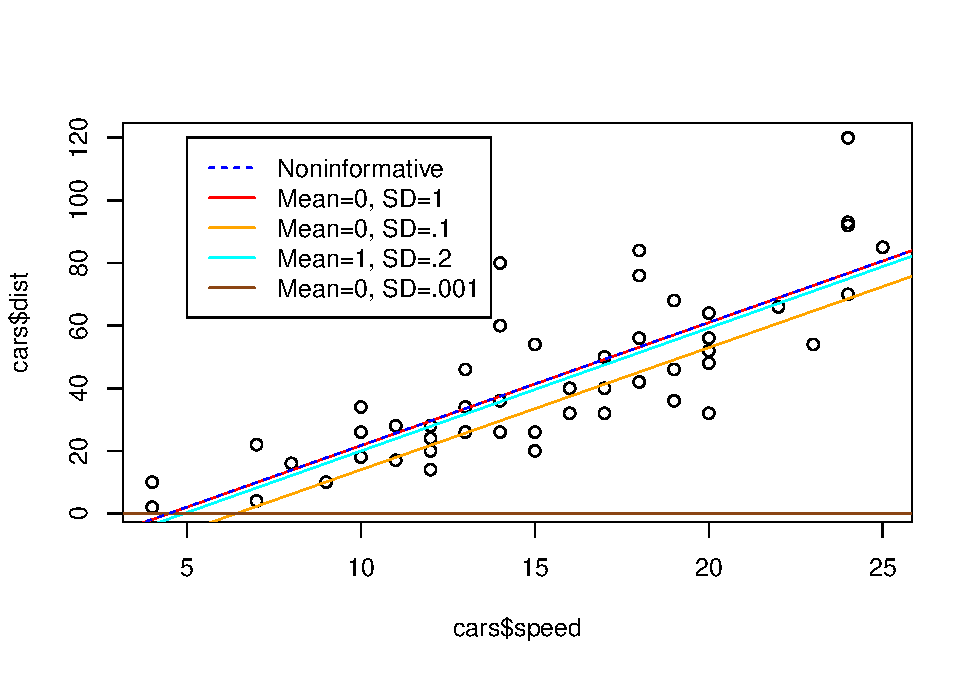
\includegraphics{ex01_files/figure-latex/unnamed-chunk-2-1.pdf}

We notice how the data strongly dominate the likelihood: in fact, by
setting the standard deviation of the prior to 1, we get the same result
of the noninformative case; however, by playing with the value for SD,
and setting it to very low values, we can see that the regression line
is shifted a bit lower (there're only slight changes in intercept). If
we set a too low SD, the prior dominates the data too much, resulting in
a flat line with extremely low values for intercept and coefficient
which does not fit the data at all.

\section{Ecercise 2.7}\label{ecercise-2.7}

\subsection{a)}\label{a}

The binomial distribution, whose pmf is

\[
Bin(n,\pi) = \binom{n}{y}\theta^y(1-\theta)^{n-y}
\] Belongs to the exponential family, and its natural parameter may be
expressed as \[
\phi(\theta) = logit(\theta) = log(\theta/(1-\theta))
\] \(\pi\) is a probability value, \(\rightarrow \in [0,1]\);
\(\phi(\pi)\) is then defined over the whole real line.

We then suppose to have a uniform constant prior for \(\phi(\theta)\),
hence \(\pi_{\phi(\theta)}(\phi(\theta)) \propto k\), with
\(k \in \mathbb{R}\).

To find the corresponding prior for \(\theta, \pi_\theta(\theta)\) we
must invert the logit function:

\[
\theta = logit(\theta)^{-1} = \frac{\exp{\phi(\theta)}}{1+\exp{\phi(\theta)}} \doteq invlogit(\theta)
\]

Then

\[
\pi_\theta(\theta) = \pi_{\phi(\theta)}(invlogit(\theta)^{-1}) \frac{\mathrm{d}\ invlogit(\theta)^{-1}}{\mathrm{d}\theta} =
\pi_{\phi(\theta)}(logit(\theta)) \frac{\mathrm{d}\ logit(\theta)}{\mathrm{d}\theta}
\propto k \cdot \frac{1}{\theta(1-\theta)} \propto   \frac{1}{\theta(1-\theta)}
\]

\subsection{b)}\label{b}

The posterior is the following \[
p(y|\theta)\cdot  \pi(\theta) \propto \theta^y(1-\theta)^{n-y}\theta^{-1}(1-\theta)^{-1} = 
\theta^{y-1}(1-\theta)^{n-y-1} 
\] Which is the core for a \(Beta(y, n-y)\).

If we consider its integral over the whole parameter space \[
\int_0^1\theta^{y-1}(1-\theta)^{n-y-1}\ d\theta
\] When \(y=0 \vee y=n\), it becomes either: \[
\int_0^1(1-\theta)^{n-1}/\theta\ d\theta
\] or \[
\int_0^1\theta^{n-1}/(1-\theta)\ d\theta
\]

We notice that, in both cases, it's an improper integral, since 0 and 1
are both vertical asymptotes for the two function respectively. To solve
the integral, we first have to consider the indefinite case, using the
decomposition \((1-\theta)^{n}=\sum_{i=0}^{n}\binom{n}{i}(-\theta)^i\):

\[
\int(1-\theta)^{n-1}/\theta\ d\theta = \int \sum_{i=0}^{n-1}\binom{n-1}{i}(-\theta)^i/\theta\ d\theta
\] We can externalize from the integral everything not containing
\(\theta\), while decomposing \((-\theta)^i\) as
\((-1\cdot\theta)^i = (-1)^i(\theta)^i\): \[
\sum_{i=0}^{n-1}\binom{n-1}{i}(-\theta)^i/\theta\ d\theta = \sum\binom{n-1}{i}(-1)^i\int\theta^{i-1}d\theta
\] The integral for \(\theta^{i-1}\) has different solutions depending
upon the value of \(i\):

\begin{enumerate}
\def\labelenumi{\arabic{enumi}.}
\tightlist
\item
  If \(i>0\), it is \(\theta^i/i\);
\item
  If \(\theta=0\), it is \(log(\theta)\)
\end{enumerate}

Unwinding the sum, then, we'll have \(n-2\) polynomial terms in
\theta and one logarithmic term in \theta. It's easy to see as, if we
bring our attention back to the definite integral, we'll have that the
logarithmic term will yield an infinite value as we approach zero, while
the polynomial part will yield real values, thus resulting in an
infinite integral for our posterior, hence its improper nature for the
extreme value \(y=0\). For the opposite case (\(y=n\)), we'll have an
analogous result since we have a \(log(1-\theta)\), which is infinite
when we approach 1.

\section{Exercise 2.8}\label{exercise-2.8}

Prior distribution:

\[ \theta \sim N(\mu_0, \tau^2_0) = N(180, 40^2) = N(180, 1600) \]

Likelihood:

\[ y_i|\theta \sim N(\theta, 400)  \]

We know that \(\bar{y}=150\).

\subsection{\texorpdfstring{a) Obtain posterior as a function of
\(n\)}{a) Obtain posterior as a function of n}}\label{a-obtain-posterior-as-a-function-of-n}

We also know that (ref. to Gelman book for proof), for a normal prior
and likelihood, with population variance known:

\[
\pi(\theta|y) = N \bigg( \frac{\mu_0/ \tau^2_0 + n \bar{y} / \sigma^2}{1/ \tau^2_0 + n / \sigma^2},
    (1/\tau^2_0+n/\sigma^2)^{-1} \bigg)
\]

Applied to our data: \[
N\bigg(\frac{180/1600+n \cdot 150/400}{1/1600+n/400}, (1/1600+n/400)^{-1} \bigg)
=
N\bigg(\frac{0.1125+n \cdot 0.3750}{1/1600+n/400}, (1/1600+n/400)^{-1}\bigg)
\]

\subsection{\texorpdfstring{b) Obtain posterior predictive as a function
of
\(n\)}{b) Obtain posterior predictive as a function of n}}\label{b-obtain-posterior-predictive-as-a-function-of-n}

We know that the posterior predictive distribution
\(\tilde{y}|y ~ N(\mu_n, \sigma^2_n+\sigma^2)\), where \(\mu_n\) and
\(\sigma^2_n\) are the mean and variance from the posterior. Hence:

\[
\tilde{y}|y \sim N\bigg(\frac{0.1125+n\cdot0.3750}{1/1600+n/400}, (1/1600+n/400)^{-1} + 400\bigg)
\]

The mean is the same of the posterior, while the posterior variance gets
enlarged encompassing also prior uncertainty.

\subsection{\texorpdfstring{c) Obtain 95\% posterior and posterior
predictive intervals with
\(n=10\)}{c) Obtain 95\% posterior and posterior predictive intervals with n=10}}\label{c-obtain-95-posterior-and-posterior-predictive-intervals-with-n10}

If \(n=10\),

\[
\theta|y \sim N\bigg( \frac{0.1125+n \cdot 0.3750}{1/1600+n/400}, (1/1600+n/400)^{-1} \bigg) = N(3.8625/0.0256, 39.0244) = N(150.8789, 39.0244)
\]

The 95\% posterior interval is hence obtained from this distribution:

\begin{Shaded}
\begin{Highlighting}[]
\KeywordTok{qnorm}\NormalTok{(.}\DecValTok{025}\NormalTok{, }\FloatTok{150.8789}\NormalTok{, }\KeywordTok{sqrt}\NormalTok{(}\FloatTok{39.0244}\NormalTok{))}
\end{Highlighting}
\end{Shaded}

\begin{verbatim}
## [1] 138.6351
\end{verbatim}

\begin{Shaded}
\begin{Highlighting}[]
\KeywordTok{qnorm}\NormalTok{(.}\DecValTok{975}\NormalTok{, }\FloatTok{150.8789}\NormalTok{, }\KeywordTok{sqrt}\NormalTok{(}\FloatTok{39.0244}\NormalTok{))}
\end{Highlighting}
\end{Shaded}

\begin{verbatim}
## [1] 163.1227
\end{verbatim}

For the predictive posterior 95\% interval, we just need to toggle the
variance of the distribution by summing the ground truth:

\begin{Shaded}
\begin{Highlighting}[]
\KeywordTok{qnorm}\NormalTok{(.}\DecValTok{025}\NormalTok{, }\FloatTok{150.8789}\NormalTok{, }\KeywordTok{sqrt}\NormalTok{(}\FloatTok{39.0244} \OperatorTok{+}\StringTok{ }\DecValTok{400}\NormalTok{))}
\end{Highlighting}
\end{Shaded}

\begin{verbatim}
## [1] 109.812
\end{verbatim}

\begin{Shaded}
\begin{Highlighting}[]
\KeywordTok{qnorm}\NormalTok{(.}\DecValTok{975}\NormalTok{, }\FloatTok{150.8789}\NormalTok{, }\KeywordTok{sqrt}\NormalTok{(}\FloatTok{39.0244} \OperatorTok{+}\StringTok{ }\DecValTok{400}\NormalTok{))}
\end{Highlighting}
\end{Shaded}

\begin{verbatim}
## [1] 191.9458
\end{verbatim}

We see how the ground truth contributes to a large increase in variance.

\subsection{\texorpdfstring{d) Same with
\(n=100\)}{d) Same with n=100}}\label{d-same-with-n100}

For \(n=100\): \$\$ \theta\textbar{}y
\sim N\bigg(\frac{0.1125+n\cdot0.3750}{1/1600+n/400},
(1/1600+n/400)\^{}\{-1\} \bigg) = N(150.0748, 3.9900)

\$\$ Then

\begin{Shaded}
\begin{Highlighting}[]
\KeywordTok{qnorm}\NormalTok{(.}\DecValTok{025}\NormalTok{, }\FloatTok{150.0784}\NormalTok{, }\KeywordTok{sqrt}\NormalTok{(}\FloatTok{3.9900}\NormalTok{))}
\end{Highlighting}
\end{Shaded}

\begin{verbatim}
## [1] 146.1634
\end{verbatim}

\begin{Shaded}
\begin{Highlighting}[]
\KeywordTok{qnorm}\NormalTok{(.}\DecValTok{975}\NormalTok{, }\FloatTok{150.0784}\NormalTok{, }\KeywordTok{sqrt}\NormalTok{(}\FloatTok{3.9900}\NormalTok{))}
\end{Highlighting}
\end{Shaded}

\begin{verbatim}
## [1] 153.9934
\end{verbatim}

and, for the posterior predictive,

\begin{Shaded}
\begin{Highlighting}[]
\KeywordTok{qnorm}\NormalTok{(.}\DecValTok{025}\NormalTok{, }\FloatTok{150.0784}\NormalTok{, }\KeywordTok{sqrt}\NormalTok{(}\FloatTok{3.9900} \OperatorTok{+}\StringTok{ }\DecValTok{400}\NormalTok{))}
\end{Highlighting}
\end{Shaded}

\begin{verbatim}
## [1] 110.6841
\end{verbatim}

\begin{Shaded}
\begin{Highlighting}[]
\KeywordTok{qnorm}\NormalTok{(.}\DecValTok{975}\NormalTok{, }\FloatTok{150.0784}\NormalTok{, }\KeywordTok{sqrt}\NormalTok{(}\FloatTok{3.9900} \OperatorTok{+}\StringTok{ }\DecValTok{400}\NormalTok{))}
\end{Highlighting}
\end{Shaded}

\begin{verbatim}
## [1] 189.4727
\end{verbatim}

We see how, increasing \(n\), the posterior and posterior predictive
mean gets pulled towards the sample mean, while the posterior variance
decreases towards zero; the posterior predictive variance instead still
remains hight due to the large value imposed by the ground truth.

\section{Lab-1}\label{lab-1}

\subsection{1. Plot priors}\label{plot-priors}

\begin{Shaded}
\begin{Highlighting}[]
\CommentTok{#Here we store all the params - each row contains a couple of params for the linked Gamma prior}
\NormalTok{params =}\StringTok{ }\KeywordTok{matrix}\NormalTok{(}\KeywordTok{c}\NormalTok{(}\DecValTok{1}\NormalTok{,.}\DecValTok{5}\NormalTok{,}\DecValTok{1}\NormalTok{,}\DecValTok{2}\NormalTok{,}\DecValTok{1}\NormalTok{,}\DecValTok{10}\NormalTok{,}\DecValTok{2}\NormalTok{,}\DecValTok{2}\NormalTok{,.}\DecValTok{5}\NormalTok{,}\DecValTok{0}\NormalTok{), }\DataTypeTok{ncol =} \DecValTok{2}\NormalTok{, }\DataTypeTok{nrow =} \DecValTok{5}\NormalTok{, }\DataTypeTok{byrow =}\NormalTok{ T)}

\KeywordTok{plot}\NormalTok{(}\OtherTok{NULL}\NormalTok{, }\DataTypeTok{xlim=}\KeywordTok{c}\NormalTok{(}\DecValTok{0}\NormalTok{,}\DecValTok{3}\NormalTok{), }\DataTypeTok{ylim=}\KeywordTok{c}\NormalTok{(}\DecValTok{0}\NormalTok{,}\DecValTok{3}\NormalTok{), }\DataTypeTok{xlab=}\StringTok{"x"}\NormalTok{, }\DataTypeTok{ylab=}\StringTok{"p(x)"}\NormalTok{, }\DataTypeTok{main =} \StringTok{"Priors for Ship Accidents data"}\NormalTok{)}

\ControlFlowTok{for}\NormalTok{(i }\ControlFlowTok{in} \DecValTok{1}\OperatorTok{:}\NormalTok{(}\KeywordTok{nrow}\NormalTok{(params)}\OperatorTok{-}\DecValTok{1}\NormalTok{))\{}
  \KeywordTok{curve}\NormalTok{(}\KeywordTok{dgamma}\NormalTok{(x,params[i,}\DecValTok{1}\NormalTok{],params[i,}\DecValTok{2}\NormalTok{]), }\DataTypeTok{add=}\NormalTok{T, }\DataTypeTok{col=}\NormalTok{i)  }
\NormalTok{\}}
\KeywordTok{curve}\NormalTok{(}\DecValTok{1}\OperatorTok{/}\KeywordTok{sqrt}\NormalTok{(x), }\DataTypeTok{add =}\NormalTok{ T, }\DataTypeTok{col=} \DecValTok{5}\NormalTok{, }\DataTypeTok{lty =} \DecValTok{5}\NormalTok{)}
\KeywordTok{legend}\NormalTok{(}\DataTypeTok{x=}\DecValTok{2}\NormalTok{, }\DataTypeTok{y=}\DecValTok{3}\NormalTok{, }\KeywordTok{c}\NormalTok{(}\StringTok{"Gamma(1,0.5)"}\NormalTok{, }\StringTok{"Gamma(1,2)"}\NormalTok{,}\StringTok{"Gamma(1,10)"}\NormalTok{,}\StringTok{"Gamma(2,2)"}\NormalTok{,}\StringTok{"Jeffreys'"}\NormalTok{), }\DataTypeTok{col=}\KeywordTok{c}\NormalTok{(}\DecValTok{1}\NormalTok{,}\DecValTok{2}\NormalTok{,}\DecValTok{3}\NormalTok{,}\DecValTok{4}\NormalTok{,}\DecValTok{5}\NormalTok{), }\DataTypeTok{lty=}\KeywordTok{c}\NormalTok{(}\KeywordTok{rep}\NormalTok{(}\DecValTok{1}\NormalTok{,}\DecValTok{4}\NormalTok{),}\DecValTok{5}\NormalTok{))}
\end{Highlighting}
\end{Shaded}

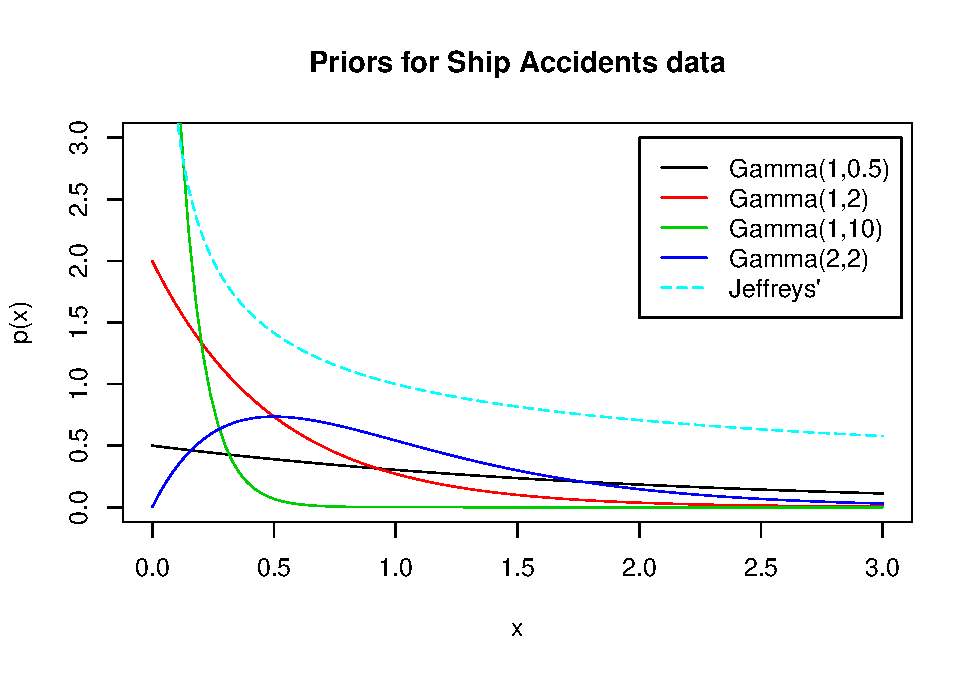
\includegraphics{ex01_files/figure-latex/unnamed-chunk-8-1.pdf}

\subsection{2. Plot posteriors for each
prior}\label{plot-posteriors-for-each-prior}

First, we have to generalize the model in the lab's slides for
observations with different exposure. As suggested by Gelman (page 45 of
textbook), we account for it by setting \(y_i\sim Poisson(t_i\theta)\),
where \(t_i\) is the exposure for unit \(i\). The likelihood becomes
then \[
p(y|\theta) \sim \theta^{\sum y_i}e^{(-\sum t_i)\theta} 
\] , which is a \(Gamma(\sum y_i +1, \sum t_i)\).

With Gamma prior, the posterior is hence:

\[
\pi(\theta|y,t) = Gamma\bigg(\alpha+\sum_i y_i, \beta + \sum_i t_i\bigg)
\]

Having a closer look at the data:

\begin{Shaded}
\begin{Highlighting}[]
\KeywordTok{head}\NormalTok{(ShipAccidents)}
\end{Highlighting}
\end{Shaded}

\begin{verbatim}
##   type construction operation service incidents
## 1    A      1960-64   1960-74     127         0
## 2    A      1960-64   1975-79      63         0
## 3    A      1965-69   1960-74    1095         3
## 4    A      1965-69   1975-79    1095         4
## 5    A      1970-74   1960-74    1512         6
## 6    A      1970-74   1975-79    3353        18
\end{verbatim}

we have that
\(t_i \rightarrow \texttt{service}; y_i \rightarrow \texttt{incidents}\).

We store in \texttt{y} the value for our count data, the incidents,
removing those values with \texttt{service} equals to 0 since they're
useless for our analysis.

\begin{Shaded}
\begin{Highlighting}[]
\NormalTok{(}\DataTypeTok{y =}\NormalTok{ ShipAccidents[ShipAccidents}\OperatorTok{$}\NormalTok{service}\OperatorTok{>}\DecValTok{0}\NormalTok{,}\StringTok{"incidents"}\NormalTok{])}
\end{Highlighting}
\end{Shaded}

\begin{verbatim}
##  [1]  0  0  3  4  6 18 11 39 29 58 53 12 44 18  1  1  0  1  6  2  1  0  0
## [24]  0  0  2 11  4  0  7  7  5 12  1
\end{verbatim}

Analogously, we define a variable \texttt{t} to store info about
exposure:

\begin{Shaded}
\begin{Highlighting}[]
\NormalTok{(}\DataTypeTok{t =}\NormalTok{ ShipAccidents[ShipAccidents}\OperatorTok{$}\NormalTok{service}\OperatorTok{>}\DecValTok{0}\NormalTok{,}\StringTok{"service"}\NormalTok{])}
\end{Highlighting}
\end{Shaded}

\begin{verbatim}
##  [1]   127    63  1095  1095  1512  3353  2244 44882 17176 28609 20370
## [12]  7064 13099  7117  1179   552   781   676   783  1948   274   251
## [23]   105   288   192   349  1208  2051    45   789   437  1157  2161
## [34]   542
\end{verbatim}

The posterior is: \[
\theta|y \sim Gamma\bigg(\alpha+\sum_iy_i; \beta + \sum_i t_i\bigg)
\]

Since \texttt{sum(t)} is very large, it would lead us to unplottable
posterior due to limitations of R. To allow for a visual analysis of our
data, we arbitrarily rescale the exposure by a factor of 5000:

\begin{Shaded}
\begin{Highlighting}[]
\NormalTok{t_new =}\StringTok{ }\NormalTok{t}\OperatorTok{/}\DecValTok{5000}
\end{Highlighting}
\end{Shaded}

Note that this leads to a different interpretation of the rate
(accidents in months of service/5000 instead of accidents in months of
service): to obtain the same results as in the original data, \texttt{y}
would have to be rescaled as well.

We plot it for each configuration of parameters (note that the x axis
doesn't begin at 0 to allow for a better zoom on the curves) adding the
likelihood in dashed line for reference:

\begin{Shaded}
\begin{Highlighting}[]
\CommentTok{#define functional for posterior}
\NormalTok{dposterior_gamma_pois =}\StringTok{ }\ControlFlowTok{function}\NormalTok{(x, alpha, beta, rate, exposure)\{}
    \KeywordTok{return}\NormalTok{ (}\KeywordTok{dgamma}\NormalTok{(x, alpha }\OperatorTok{+}\StringTok{ }\KeywordTok{sum}\NormalTok{(rate), beta }\OperatorTok{+}\StringTok{ }\KeywordTok{sum}\NormalTok{(exposure)))}
\NormalTok{\}}

\CommentTok{#for-cycle plotting}
\KeywordTok{plot}\NormalTok{(}\OtherTok{NULL}\NormalTok{, }\DataTypeTok{xlim=}\KeywordTok{c}\NormalTok{(}\FloatTok{6.75}\NormalTok{,}\DecValTok{14}\NormalTok{), }\DataTypeTok{ylim=}\KeywordTok{c}\NormalTok{(}\DecValTok{0}\NormalTok{,}\DecValTok{1}\NormalTok{), }\DataTypeTok{xlab=}\StringTok{"x"}\NormalTok{, }\DataTypeTok{ylab=}\StringTok{"p(x)"}\NormalTok{, }\DataTypeTok{main=}\StringTok{"Posteriors and likelihood for ship accidents data"}\NormalTok{)}

\ControlFlowTok{for}\NormalTok{(i }\ControlFlowTok{in} \DecValTok{1}\OperatorTok{:}\KeywordTok{nrow}\NormalTok{(params))\{}
  \KeywordTok{curve}\NormalTok{(}\KeywordTok{dposterior_gamma_pois}\NormalTok{(x, params[i,}\DecValTok{1}\NormalTok{], params[i,}\DecValTok{2}\NormalTok{], y, t_new), }\DataTypeTok{add=}\NormalTok{T, }\DataTypeTok{col=}\NormalTok{i)  }
\NormalTok{\}}
\KeywordTok{curve}\NormalTok{(}\KeywordTok{dgamma}\NormalTok{(x, }\KeywordTok{sum}\NormalTok{(y)}\OperatorTok{+}\DecValTok{1}\NormalTok{, }\KeywordTok{sum}\NormalTok{(t_new)), }\DataTypeTok{add =}\NormalTok{ T, }\DataTypeTok{col =} \StringTok{"orange"}\NormalTok{, }\DataTypeTok{lwd=}\DecValTok{2}\NormalTok{, }\DataTypeTok{lty=}\DecValTok{5}\NormalTok{)}
\KeywordTok{legend}\NormalTok{(}\DataTypeTok{x=}\FloatTok{11.5}\NormalTok{, }\DataTypeTok{y=}\DecValTok{1}\NormalTok{, }\KeywordTok{c}\NormalTok{(}\StringTok{"pr. Gamma(1,0.5)"}\NormalTok{, }\StringTok{"pr. Gamma(1,2)"}\NormalTok{,}\StringTok{"pr. Gamma(1,10)"}\NormalTok{,}\StringTok{"pr. Gamma(2,2)"}\NormalTok{,}\StringTok{"Jeffreys' pr."}\NormalTok{, }\StringTok{"likelihood"}\NormalTok{), }\DataTypeTok{col=}\KeywordTok{c}\NormalTok{(}\DecValTok{1}\NormalTok{,}\DecValTok{2}\NormalTok{,}\DecValTok{3}\NormalTok{,}\DecValTok{4}\NormalTok{,}\DecValTok{5}\NormalTok{,}\StringTok{"orange"}\NormalTok{), }\DataTypeTok{lty=}\KeywordTok{c}\NormalTok{(}\KeywordTok{rep}\NormalTok{(}\DecValTok{1}\NormalTok{,}\DecValTok{5}\NormalTok{),}\DecValTok{5}\NormalTok{))}
\end{Highlighting}
\end{Shaded}

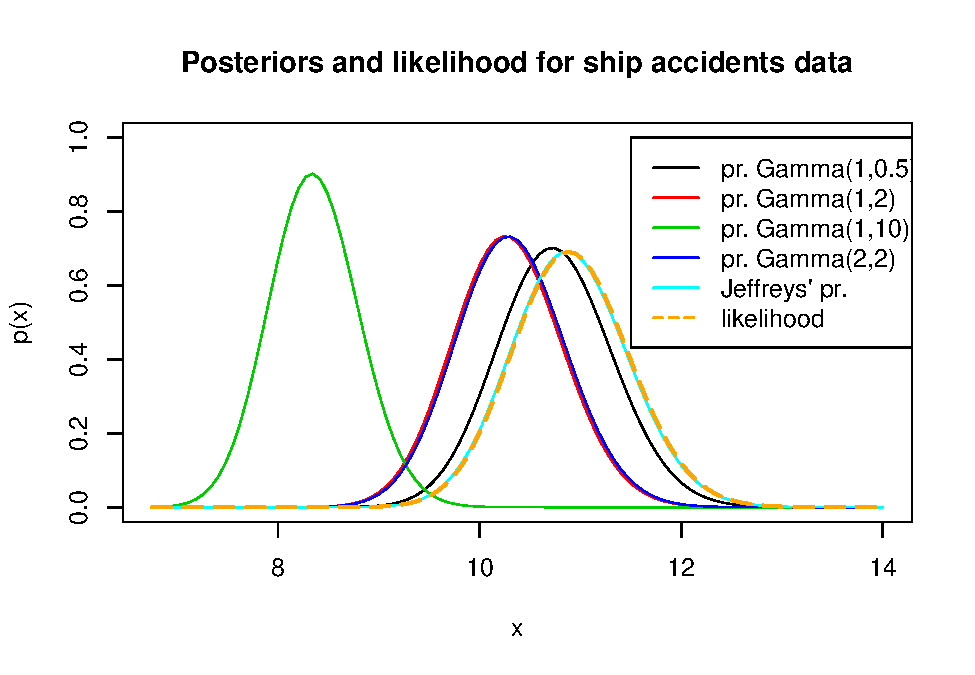
\includegraphics{ex01_files/figure-latex/unnamed-chunk-13-1.pdf}

\subsection{3. Find posterior expectation and
MAP}\label{find-posterior-expectation-and-map}

The expected value for the gamma posterior is
\(\frac{\sum y_i + \alpha}{n+\beta}\), while the MAP is
\(\frac{\sum y_i + \alpha-1}{n+\beta}\).

\begin{Shaded}
\begin{Highlighting}[]
\ControlFlowTok{for}\NormalTok{(i }\ControlFlowTok{in} \DecValTok{1}\OperatorTok{:}\KeywordTok{nrow}\NormalTok{(params))\{}
  \KeywordTok{print}\NormalTok{(}\KeywordTok{paste0}\NormalTok{(}\StringTok{"Prior alpha = "}\NormalTok{, params[i,}\DecValTok{1}\NormalTok{], }\StringTok{", beta = "}\NormalTok{, params[i,}\DecValTok{2}\NormalTok{]))}
  \KeywordTok{print}\NormalTok{(}\KeywordTok{paste0}\NormalTok{(}\StringTok{"    Exp. value: "}\NormalTok{, (}\KeywordTok{sum}\NormalTok{(y)}\OperatorTok{+}\NormalTok{params[i,}\DecValTok{1}\NormalTok{])}\OperatorTok{/}\NormalTok{(}\KeywordTok{sum}\NormalTok{(t_new)}\OperatorTok{+}\NormalTok{params[i,}\DecValTok{2}\NormalTok{]) ))}
  \KeywordTok{print}\NormalTok{(}\KeywordTok{paste0}\NormalTok{(}\StringTok{"    MAP: "}\NormalTok{, (}\KeywordTok{sum}\NormalTok{(y)}\OperatorTok{+}\NormalTok{params[i,}\DecValTok{1}\NormalTok{]}\OperatorTok{-}\DecValTok{1}\NormalTok{)}\OperatorTok{/}\NormalTok{(}\KeywordTok{sum}\NormalTok{(t_new)}\OperatorTok{+}\NormalTok{params[i,}\DecValTok{2}\NormalTok{]) ))}
\NormalTok{\}}
\end{Highlighting}
\end{Shaded}

\begin{verbatim}
## [1] "Prior alpha = 1, beta = 0.5"
## [1] "    Exp. value: 10.7482206727122"
## [1] "    MAP: 10.7181136120043"
## [1] "Prior alpha = 1, beta = 2"
## [1] "    Exp. value: 10.2837982647171"
## [1] "    MAP: 10.2549921071128"
## [1] "Prior alpha = 1, beta = 10"
## [1] "    Exp. value: 8.35775890323729"
## [1] "    MAP: 8.33434781387248"
## [1] "Prior alpha = 2, beta = 2"
## [1] "    Exp. value: 10.3126044223213"
## [1] "    MAP: 10.2837982647171"
## [1] "Prior alpha = 0.5, beta = 0"
## [1] "    Exp. value: 10.8972086028342"
## [1] "    MAP: 10.8666413977772"
\end{verbatim}

\subsection{4. Comments}\label{comments}

We see that the posteriors seem pretty simmetric (as confirmed by the
means and MAP being very close to each other) concentrated with spikes
around 10 and 11.

The \(Gamma(1,10)\) (the most informative prior), is the one which
yields the most informative posterior as well, having a very steep and
narrow bell shape; however, it's the one whose mean and MAP are farther
away from our likelihood.

The \(Gamma(2,2)\) and \(Gamma(1,2)\) yield pretty undistinguishable
posteriors simmetrically located around 10.

The other two priors, \(Gamma(1, 0.5)\) and Jeffreys', are those which
get farther to the right, and are also those which yield less
informative posteriors, having a larger bell shape than the other
posteriors. We see how the Jeffreys', as expected, is the posterior
which is closer to the likelihood, being merely distinguishable from it.

\subsection{5. Construct the 95\% credible intervals, equi-tails and
highest posterior density (HPD), using the Jeffreys’
prior.}\label{construct-the-95-credible-intervals-equi-tails-and-highest-posterior-density-hpd-using-the-jeffreysa-prior.}

The credible interval can be obtained from the quantiles of the
theoretical gamma posterior:

\begin{Shaded}
\begin{Highlighting}[]
\NormalTok{(}\DataTypeTok{cred =} \KeywordTok{qgamma}\NormalTok{(}\KeywordTok{c}\NormalTok{(.}\DecValTok{025}\NormalTok{,.}\DecValTok{975}\NormalTok{),.}\DecValTok{5}\OperatorTok{+}\KeywordTok{sum}\NormalTok{(y),}\KeywordTok{sum}\NormalTok{(t_new)))}
\end{Highlighting}
\end{Shaded}

\begin{verbatim}
## [1]  9.795248 12.057061
\end{verbatim}

To construct the HPD, as done during lab, we simulate 1000 observations
from the theoretical gamma

\begin{Shaded}
\begin{Highlighting}[]
\KeywordTok{set.seed}\NormalTok{(}\DecValTok{1}\NormalTok{)}
\NormalTok{hpd<-}\ControlFlowTok{function}\NormalTok{(y,p)\{}
\NormalTok{  dy<-}\KeywordTok{density}\NormalTok{(y)}
\NormalTok{  md<-dy}\OperatorTok{$}\NormalTok{x[dy}\OperatorTok{$}\NormalTok{y}\OperatorTok{==}\KeywordTok{max}\NormalTok{(dy}\OperatorTok{$}\NormalTok{y)]}
\NormalTok{  py<-dy}\OperatorTok{$}\NormalTok{y}\OperatorTok{/}\KeywordTok{sum}\NormalTok{(dy}\OperatorTok{$}\NormalTok{y)}
\NormalTok{  pys<-}\OperatorTok{-}\KeywordTok{sort}\NormalTok{(}\OperatorTok{-}\NormalTok{py)}
\NormalTok{  ct<-}\KeywordTok{min}\NormalTok{(pys[}\KeywordTok{cumsum}\NormalTok{(pys)}\OperatorTok{<}\StringTok{ }\NormalTok{p])}
  \KeywordTok{list}\NormalTok{(}\DataTypeTok{hpdr=}\KeywordTok{range}\NormalTok{(dy}\OperatorTok{$}\NormalTok{x[py}\OperatorTok{>=}\NormalTok{ct]),}\DataTypeTok{mode=}\NormalTok{md)}
\NormalTok{\}}
\NormalTok{(}\DataTypeTok{hpd_int =} \KeywordTok{hpd}\NormalTok{(}\KeywordTok{rgamma}\NormalTok{(}\DecValTok{1000}\NormalTok{, .}\DecValTok{5}\OperatorTok{+}\KeywordTok{sum}\NormalTok{(y),}\KeywordTok{sum}\NormalTok{(t_new)), .}\DecValTok{95}\NormalTok{))}
\end{Highlighting}
\end{Shaded}

\begin{verbatim}
## $hpdr
## [1]  9.781527 12.046527
## 
## $mode
## [1] 10.7994
\end{verbatim}

We can plot those two intervals as well:

\begin{Shaded}
\begin{Highlighting}[]
\KeywordTok{curve}\NormalTok{(}\KeywordTok{dposterior_gamma_pois}\NormalTok{(x, params[}\DecValTok{5}\NormalTok{,}\DecValTok{1}\NormalTok{], params[}\DecValTok{5}\NormalTok{,}\DecValTok{2}\NormalTok{], y, t_new), }\DataTypeTok{xlim=}\KeywordTok{c}\NormalTok{(}\DecValTok{8}\NormalTok{,}\DecValTok{14}\NormalTok{), }\DataTypeTok{ylim=}\KeywordTok{c}\NormalTok{(}\DecValTok{0}\NormalTok{,.}\DecValTok{75}\NormalTok{), }\DataTypeTok{xlab=}\StringTok{"x"}\NormalTok{, }\DataTypeTok{ylab=}\StringTok{"p(x)"}\NormalTok{, }\DataTypeTok{lwd=}\DecValTok{3}\NormalTok{, }\DataTypeTok{main =}\StringTok{"95% credible and HPD interval for posterior"}\NormalTok{)}

\KeywordTok{segments}\NormalTok{(cred[}\DecValTok{1}\NormalTok{],}\DecValTok{0}\NormalTok{, cred[}\DecValTok{1}\NormalTok{], }\KeywordTok{dposterior_gamma_pois}\NormalTok{(cred[}\DecValTok{1}\NormalTok{], params[}\DecValTok{5}\NormalTok{,}\DecValTok{1}\NormalTok{], params[}\DecValTok{5}\NormalTok{,}\DecValTok{2}\NormalTok{], y, t_new), }\DataTypeTok{col=}\StringTok{"red"}\NormalTok{, }\DataTypeTok{lwd=}\DecValTok{2}\NormalTok{)}

\KeywordTok{segments}\NormalTok{(cred[}\DecValTok{2}\NormalTok{],}\DecValTok{0}\NormalTok{, cred[}\DecValTok{2}\NormalTok{], }\KeywordTok{dposterior_gamma_pois}\NormalTok{(cred[}\DecValTok{2}\NormalTok{], params[}\DecValTok{5}\NormalTok{,}\DecValTok{1}\NormalTok{], params[}\DecValTok{5}\NormalTok{,}\DecValTok{2}\NormalTok{], y, t_new), }\DataTypeTok{col=}\StringTok{"red"}\NormalTok{, }\DataTypeTok{lwd=}\DecValTok{2}\NormalTok{)}

\KeywordTok{segments}\NormalTok{(cred[}\DecValTok{1}\NormalTok{], .}\DecValTok{09}\NormalTok{, cred[}\DecValTok{2}\NormalTok{], .}\DecValTok{09}\NormalTok{, }\DataTypeTok{col=}\StringTok{"red"}\NormalTok{)}

\KeywordTok{text}\NormalTok{(}\KeywordTok{mean}\NormalTok{(cred), .}\DecValTok{12}\NormalTok{, }\StringTok{"95% credible interval"}\NormalTok{, }\DataTypeTok{col=}\StringTok{"red"}\NormalTok{)}

\KeywordTok{segments}\NormalTok{(hpd_int}\OperatorTok{$}\NormalTok{hpdr[}\DecValTok{1}\NormalTok{],}\DecValTok{0}\NormalTok{, hpd_int}\OperatorTok{$}\NormalTok{hpdr[}\DecValTok{1}\NormalTok{], }\KeywordTok{dposterior_gamma_pois}\NormalTok{(hpd_int}\OperatorTok{$}\NormalTok{hpdr[}\DecValTok{1}\NormalTok{], params[}\DecValTok{5}\NormalTok{,}\DecValTok{1}\NormalTok{], params[}\DecValTok{5}\NormalTok{,}\DecValTok{2}\NormalTok{], y, t_new), }\DataTypeTok{col=}\StringTok{"blue"}\NormalTok{, }\DataTypeTok{lwd=}\DecValTok{2}\NormalTok{)}

\KeywordTok{segments}\NormalTok{(hpd_int}\OperatorTok{$}\NormalTok{hpdr[}\DecValTok{2}\NormalTok{],}\DecValTok{0}\NormalTok{, hpd_int}\OperatorTok{$}\NormalTok{hpdr[}\DecValTok{2}\NormalTok{], }\KeywordTok{dposterior_gamma_pois}\NormalTok{(hpd_int}\OperatorTok{$}\NormalTok{hpdr[}\DecValTok{2}\NormalTok{], params[}\DecValTok{5}\NormalTok{,}\DecValTok{1}\NormalTok{], params[}\DecValTok{5}\NormalTok{,}\DecValTok{2}\NormalTok{], y, t_new), }\DataTypeTok{col=}\StringTok{"blue"}\NormalTok{, }\DataTypeTok{lwd=}\DecValTok{2}\NormalTok{)}

\KeywordTok{segments}\NormalTok{(hpd_int}\OperatorTok{$}\NormalTok{hpdr[}\DecValTok{1}\NormalTok{], .}\DecValTok{05}\NormalTok{, hpd_int}\OperatorTok{$}\NormalTok{hpdr[}\DecValTok{2}\NormalTok{], .}\DecValTok{05}\NormalTok{, }\DataTypeTok{col=}\StringTok{"blue"}\NormalTok{)}

\KeywordTok{text}\NormalTok{(}\KeywordTok{mean}\NormalTok{(hpd_int}\OperatorTok{$}\NormalTok{hpdr), .}\DecValTok{03}\NormalTok{, }\StringTok{"95% HPD interval"}\NormalTok{, }\DataTypeTok{col=}\StringTok{"blue"}\NormalTok{)}
\end{Highlighting}
\end{Shaded}

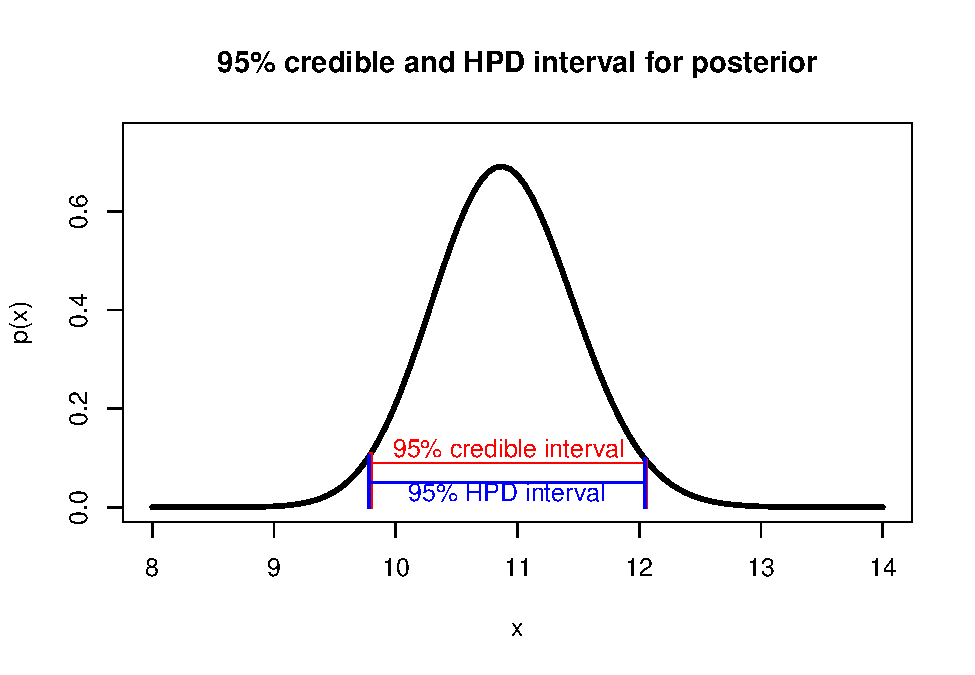
\includegraphics{ex01_files/figure-latex/unnamed-chunk-17-1.pdf}

Since the distribution is very symmetric, the two intervals almost
coincide (note that the 95\% HPD interval should be plotted inside the
histogram of the simulated observations from where it was obtained,
plotting it here isn't 100\% correct).


\end{document}
